\section*{7. Diseño del sistema}
El presente capítulo describe el diseño integral del sistema desarrollado,
abordando de forma estructurada tanto la arquitectura software como la
organización de los datos y la experiencia de usuario. Se parte de una visión
global del sistema para, posteriormente, profundizar en los distintos niveles de
abstracción, incluyendo la arquitectura, el modelado de datos, los patrones de
diseño y la interfaz de usuario.
 
El objetivo principal de este diseño es garantizar un sistema robusto, escalable
y mantenible, capaz de integrar de forma eficiente componentes heterogéneos como
servicios web, procesamiento de datos y modelos de Machine Learning. Para ello,
se ha seguido un enfoque basado en buenas prácticas de ingeniería del software,
priorizando la separación de responsabilidades, la modularidad y la
reutilización de componentes.
 
\subsection{7.1 Arquitectura global del sistema}
La arquitectura del sistema define la organización de sus componentes
principales, así como las relaciones e interacciones entre ellos, estableciendo
las bases para su correcto funcionamiento y evolución futura. En este proyecto,
se ha optado por una arquitectura distribuida que separa claramente las capas de
frontend, backend y sistemas de datos, favoreciendo la escalabilidad,
flexibilidad y mantenibilidad del sistema.
 
Esta separación permite desacoplar responsabilidades y facilitar la evolución
independiente de cada componente. En particular, la capa de datos queda
especializada en tres subsistemas complementarios: persistencia transaccional en
PostgreSQL, búsqueda y recuperación documental en MeiliSearch, y almacenamiento
en memoria de baja latencia mediante Redis. Esta distribución funcional reduce
cuellos de botella en lectura, mejora la capacidad de respuesta del sistema y
habilita comunicación asíncrona eficiente para funcionalidades en tiempo real.
 
\begin{figure}[H]
\centering
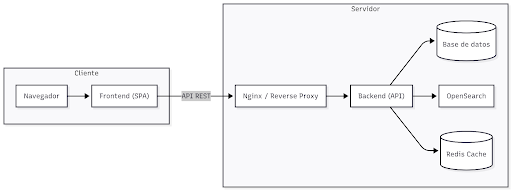
\includegraphics[width=0.8\textwidth]{images/altonivel.png}
\caption{Resumen de alto nivel de la arquitectura.}
\label{fig:altonivel}
\end{figure}
 
Este diagrama representa la arquitectura física y lógica del sistema, detallando
cómo interactúan los componentes del lado del cliente y del servidor. A
continuación, se presenta una explicación técnica y formal de cada bloque,
adecuada para la memoria de un TFG.
 
\subsubsection{Bloque de cliente: frontend}
 
A diferencia de una arquitectura monolítica tradicional, el cliente actúa como
un nodo independiente que se ejecuta en el navegador del usuario.
 
El frontend es la capa de presentación encargada de renderizar la interfaz de
usuario. Aunque consume recursos de forma dinámica, su función principal es
capturar las interacciones del usuario y presentar los datos procesados
(estadísticas, predicciones y gráficos XAI) de manera comprensible. El
navegador descarga los activos del frontend y establece una conexión de red con
el servidor a través de protocolos estándar.
 
\subsubsection{Punto de entrada: Nginx}
 
Nginx se configura como el punto de entrada principal al servidor, actuando como intermediario
entre el cliente y los servicios internos. Su incorporación responde a decisiones de diseño
centradas tanto en la mejora del rendimiento como en el refuerzo de la seguridad, ya que permite
gestionar de forma eficiente el flujo de peticiones que llegan desde el frontend.
 
En este sentido, Nginx funciona como un proxy inverso, recibiendo las solicitudes y
redirigiéndolas al backend correspondiente de manera transparente. Además, aporta una capa
de aislamiento que protege la infraestructura interna, ocultando la topología de la red y
centralizando la gestión de políticas de seguridad, como la configuración de HTTPS/SSL,
en un único punto.
 
\subsubsection{Núcleo del sistema: backend}
El backend constituye la capa de aplicación desarrollada en Django y actúa como el núcleo que
conecta y coordina el resto de servicios del sistema. En él se implementa la lógica de negocio,
encargándose del procesamiento de las peticiones, la gestión de la autenticación
y la comunicación con el motor de Machine Learning para la obtención de predicciones y recomendaciones.
 
Asimismo, desempeña un papel de intermediación, ya que traduce las solicitudes del usuario
en consultas específicas dirigidas a los distintos sistemas de almacenamiento y búsqueda.
De este modo, se abstrae la complejidad de los servicios subyacentes y se ofrece una interfaz unificada
y coherente al frontend.
 
La solución propuesta se fundamenta en una arquitectura distribuida, en la que
las responsabilidades de presentación, orquestación, lógica de negocio y
persistencia se encuentran claramente separadas. Este enfoque permite garantizar
propiedades clave como la escalabilidad, mantenibilidad y extensibilidad,
aspectos críticos en sistemas que integran componentes web y modelos de Machine
Learning.
 
\subsubsection{7.1.2 Patrones empleados}
Con el objetivo de estructurar el sistema de forma clara, mantenible y
escalable, se han aplicado diversos patrones de diseño arquitectónicos
ampliamente utilizados en la ingeniería del software. Estos patrones permiten
organizar el código de manera eficiente, reducir el acoplamiento entre
componentes y facilitar tanto la evolución como la reutilización del sistema.
A continuación, se describen los principales patrones adoptados, junto con su
aplicación concreta dentro del proyecto y la justificación de su uso desde un
punto de vista técnico.
 
\subsubsection{Modelo MVC / MTV}
 
El sistema adopta el patrón clásico Model-View-Controller (MVC), adaptado al
framework Django bajo la variante Model-Template-View (MTV). Este patrón
establece una separación clara entre la representación de los datos, la lógica
de control y la presentación.
 
\textbf{Aplicación en el sistema:}
\begin{itemize}
\item \texttt{models.py}: define el modelo de dominio, incluyendo las entidades
persistentes y sus relaciones.
\item \texttt{main/api/*} y \texttt{drf\_views.py}: implementan la capa de
control, gestionando las peticiones HTTP y exponiendo la API REST.
\item \texttt{frontend-web/src/*}: constituye la capa de presentación,
desarrollada en React.
\end{itemize}
 
Este patrón permite desacoplar la lógica de negocio de la interfaz de usuario y
del protocolo HTTP, facilitando la testabilidad, el mantenimiento y la evolución
del sistema a lo largo del desarrollo del proyecto.
 
\subsubsection{Patrón cliente-servidor}
 
El sistema se fundamenta en un modelo de desacoplamiento integral entre la
interfaz de usuario y la lógica de servidor. Esta separación permite que el
frontend (desarrollado en React) y el backend (Django) operen como entidades
independientes.
 
\textbf{Ventajas:}
\begin{itemize}
\item Facilita el despliegue independiente de ambas partes.
\item Permite el escalado horizontal específico (por ejemplo, aumentar instancias
de la API sin afectar al servidor de archivos estáticos).
\item Asegura que el backend pueda dar servicio a otros posibles clientes en el
futuro (como una aplicación móvil nativa) sin modificaciones estructurales.
\end{itemize}
 
\subsubsection{Arquitectura en capas}
 
El sistema se estructura siguiendo una arquitectura en capas, donde cada nivel
tiene una responsabilidad bien definida y se comunica únicamente con capas
adyacentes.
 
\textbf{Capas principales:}
\begin{itemize}
\item \textbf{Capa de presentación}: frontend-web (React).
\item \textbf{Capa de servicios/API}: api/views (Django REST Framework).
\item \textbf{Capa de lógica de negocio}: módulos de dominio y
entrenamientoModelos (ML).
\item \textbf{Capa de persistencia}: models.py y base de datos relacional.
\end{itemize}
 
La separación por capas reduce el acoplamiento entre componentes y mejora la
modularidad del sistema, siendo especialmente relevante en un entorno híbrido
que combina procesamiento de datos, modelos predictivos y servicios web.
 
\subsubsection{7.1.3 Patrones de comportamiento}
Además de los patrones arquitectónicos, el sistema incorpora patrones de
comportamiento que permiten gestionar de forma eficiente la interacción entre
componentes y la ejecución de procesos complejos. Estos patrones resultan
especialmente relevantes en contextos donde existen eventos, flujos dinámicos o
múltiples estrategias de ejecución.
En este apartado se detallan los patrones de comportamiento implementados,
poniendo especial énfasis en su utilidad dentro del sistema y en cómo
contribuyen a mejorar la extensibilidad y desacoplamiento.
 
\subsubsection{Observer}
 
El patrón Observer define una relación uno-a-muchos donde múltiples objetos
(observadores) son notificados automáticamente ante cambios de estado en un
objeto sujeto.
 
\textbf{Aplicación en el sistema:}
 
Se implementa mediante el sistema de signals de Django (\texttt{signals.py}):
\begin{itemize}
\item Creación automática de UserProfile tras la creación de un User.
\item Indexación de entidades (Jugador, Equipo) en MeiliSearch.
\item Emisión de notificaciones en tiempo real mediante WebSockets (Django
Channels), utilizando Redis como backend.
\end{itemize}
 
Este patrón desacopla la lógica de persistencia de las acciones derivadas
(indexación y notificaciones), mejorando la posible escalada del sistema.
 
\subsubsection{Template method}
 
Define el esqueleto de un algoritmo en una clase base, delegando ciertos pasos
en subclases que pueden redefinir comportamientos específicos.
 
\textbf{Aplicación en el sistema:}
\begin{itemize}
\item \texttt{common\_trainer.py}: define la clase base BaseTrainer con la
estructura del proceso de entrenamiento.
\item Scripts como \texttt{entrenar-modelo-*.py} y \texttt{predecir.py}
extienen dicha clase, sobrescribiendo etapas concretas del pipeline.
\end{itemize}
 
Permite centralizar la lógica común del entrenamiento de modelos, reduciendo
duplicidad de código y asegurando la consistencia en el pipeline de Machine
Learning.
 
\subsubsection{Strategy}
 
Permite seleccionar dinámicamente un algoritmo o comportamiento en tiempo de
ejecución.
 
\textbf{Aplicación en el sistema:}
\begin{itemize}
\item \texttt{predecir.py}: el diccionario MODELO\_POR\_POSICION determina el
modelo a utilizar según el contexto.
\item La función \texttt{cargar\_modelo(...)} selecciona la implementación
concreta.
\item \texttt{predicciones.py}: permite especificar el tipo de modelo mediante
parámetros en la petición.
\end{itemize}
 
Este patrón facilita la experimentación y comparación entre distintos algoritmos
(Random Forest, Ridge, Baseline), permitiendo cambiar la estrategia sin
modificar el flujo principal de ejecución.
 
\subsubsection{7.1.4 Patrones en el frontend}
El diseño del frontend no solo responde a criterios visuales, sino también a
principios estructurales que facilitan la gestión del estado y la reutilización
de lógica. En este sentido, se han adoptado patrones propios del ecosistema
React que permiten construir interfaces modernas, escalables y mantenibles.
A continuación, se describen los principales mecanismos utilizados en el
frontend, centrados en la gestión del estado global y la encapsulación de lógica
reutilizable.
 
\subsubsection{Hooks}
 
Los Hooks son funciones especializadas que permiten guardar el estado y otras funcionalidades
del ciclo de vida del framework dentro de componentes funcionales. A continuación, se describen
los tipos de Hooks integrados en el sistema y su propósito específico:
\begin{itemize}
\item \texttt{AuthContext.jsx} (useState, useEffect, useCallback, useContext).
\item \texttt{JornadaContext.jsx}.
\item \texttt{useTourWithManualExit.js}.
\end{itemize}
 
Más allá de los hooks nativos, el sistema implementa Custom Hooks, como useTourWithManualExit.js.
Estos son ganchos personalizados que encapsulan lógica compleja y específica del dominio para ser
reutilizada en diferentes pantallas de la aplicación. En lugar de duplicar el código del tour guiado
en cada página, el Custom Hook extrae esa lógica, manteniendo los componentes de la interfaz limpios
y centrados exclusivamente en la representación visual.
 
Esta arquitectura basada en Hooks no solo mejora la legibilidad del código, sino que asegura que el
frontend sea reactivo y eficiente, alineándose con los estándares actuales de la industria y
garantizando una experiencia de usuario fluida.
 
\subsubsection{Context API}
 
Context API es un sistema nativo de React diseñado para compartir datos de forma global entre componentes,
eliminando la necesidad de pasar propiedades manualmente a través de niveles intermedios.
Este enfoque resuelve eficazmente el prop drilling, práctica ineficiente en la que los datos deben atravesar
componentes que no los requieren funcionalmente solo para alcanzar a un nodo inferior en la jerarquía.
 
\textbf{Aplicación en el sistema:}
\begin{itemize}
\item \textbf{AuthContext}: autenticación.
\item \textbf{JornadaContext}: estado de jornada.
\item \textbf{TourContext}: gestión del tour interactivo.
\end{itemize}
 
Permite compartir información global entre componentes de forma eficiente,
mejorando la escalabilidad y mantenibilidad del frontend.
 
\subsection{7.2 Modelado predictivo}
Una vez procesados los datos, el sistema aborda la fase de modelado mediante
técnicas de Machine Learning supervisado. El objetivo es predecir el rendimiento
futuro de los jugadores a partir de su histórico y de variables contextuales.
En este apartado se describen los algoritmos utilizados, las estrategias de
optimización y las métricas empleadas para evaluar el rendimiento de los
modelos, justificando cada decisión desde un punto de vista técnico y práctico.
 
\begin{itemize}
\item \textbf{Variable objetivo ($Y$)}: \texttt{target\_pf\_next} (Puntos Fantasy
que el jugador obtendrá en la jornada siguiente).
\item \textbf{Variables independientes ($X$)}: Más de 50 variables que incluyen
medias móviles, roles de élite, dificultad del rival, localía y cuotas de
mercado.
\end{itemize}
 
\subsubsection{7.2.1 Algoritmos y optimización}
No se utiliza un único modelo, sino que se compite entre varias familias de
algoritmos para cada posición:
 
\begin{itemize}
\item \textbf{Random Forest (RF)}: Excelente para capturar interacciones no
lineales y reducir la varianza.
\item \textbf{XGBoost (XGB)}: Un algoritmo de Gradient Boosting extremadamente
potente que optimiza el error de forma iterativa.
\item \textbf{Ridge y ElasticNet}: Modelos lineales con regularización $L1$ y
$L2$ para evitar el sobreajuste cuando hay muchas variables
correlacionadas.
\end{itemize}
 
El proceso de GridSearch permite encontrar la combinación óptima de
hiperparámetros (profundidad del árbol, tasa de aprendizaje, número de
estimadores) mediante validación cruzada, seleccionando el modelo con el menor
Error Absoluto Medio (MAE).
 
\subsubsection{7.2.2 Métricas de evaluación del modelo}
Con el propósito de garantizar la validez científica y la utilidad práctica del
sistema, la evaluación del rendimiento de los modelos se ha articulado en torno
a dos métricas fundamentales: el Error Absoluto Medio (MAE) y el coeficiente de
correlación de Spearman. La elección del MAE responde a su alta
interpretabilidad en el dominio del Fantasy Football, ya que permite cuantificar
la desviación media de las predicciones en la misma unidad de medida que la
variable objetivo (puntos).
 
Complementariamente, el coeficiente de Spearman resulta crítico para validar la
capacidad de ordenación del modelo, asegurando que la jerarquía de
recomendaciones de jugadores sea consistente con su rendimiento real. Para
contextualizar estos valores, se han realizado análisis estadísticos
preliminares y procesos de benchmarking destinados a establecer umbrales de
aceptación, los cuales definen el nivel de precisión mínimo para considerar un
resultado como satisfactorio y apto para el apoyo a la decisión.
 
\subsubsection{7.2.2.1 Justificación técnica del coeficiente de Spearman}
A diferencia de la correlación de Pearson, que evalúa la relación lineal entre
dos variables, el coeficiente de correlación de Spearman ($r_s$ o
$\rho$) es una métrica adimensional que mide la fuerza y la dirección de la
asociación monótona entre dos variables. En el contexto de este proyecto, su uso
es preferible por las siguientes razones:
 
\begin{enumerate}
\item \textbf{Evaluación del ranking sobre el valor absoluto}
 
En un sistema de recomendación para mánagers, a menudo es más valioso saber qué
jugador rendirá mejor que otro (orden), que conocer la cifra exacta de puntos
(magnitud). Si el modelo predice que el Jugador A sacará 8 puntos y el Jugador B
sacará 6, y la realidad es que el A saca 5 y el B saca 3, el MAE registrará un
error alto, pero la correlación de Spearman será perfecta (+1), ya que el orden
de recomendación fue correcto para la toma de decisiones (fichar al Jugador A).
 
\item \textbf{Robustez ante relaciones no lineales}
 
Los puntos no siempre siguen una distribución lineal respecto a
las variables independientes (por ejemplo, el número de entradas o pases clave).
Spearman captura relaciones monótonas donde las variables tienden a cambiar
juntas, pero no necesariamente a un ritmo constante, lo que se ajusta mejor a la
naturaleza estocástica del deporte.
 
\item \textbf{Formulación matemática}
 
El coeficiente se calcula basándose en los rangos (posiciones en la lista) de
los datos en lugar de sus valores brutos. La fórmula utilizada es:
$$r_s = 1 - \frac{6 \sum d_i^2}{n(n^2 - 1)}$$
Donde:
\begin{itemize}
\item $d_i$: Representa la diferencia entre los rangos de la predicción y el
resultado real para cada observación $i$.
\item $n$: Es el número total de observaciones (jugadores evaluados).
\end{itemize}
 
\item \textbf{Interpretación de resultados}
 
El valor de $r_s$ oscila entre -1 y +1:
\begin{itemize}
\item $+1$: existe una coincidencia perfecta en el orden de los rangos (el
modelo ordena a los jugadores exactamente igual que su rendimiento real).
\item $0$: no existe asociación entre los rangos (las predicciones son
equivalentes al azar).
\item $-1$: existe una oposición perfecta (el modelo recomienda como ``mejores''
a los jugadores que acaban rindiendo peor).
\end{itemize}
 
En el ámbito de la analítica deportiva, debido a la alta variabilidad del juego,
se han establecido como umbrales de éxito valores de $r_s \geq X$ para
considerar que el modelo aporta un valor estadístico significativo para la
recomendación estratégica.
\end{enumerate}
 
\subsubsection{7.2.3 Criterios de validez y benchmarking de modelos}
Para determinar si un modelo predictivo es útil en un entorno tan volátil como
el fútbol, no es suficiente con obtener un error bajo; es imperativo establecer
qué constituye un ``buen resultado'' para cada posición. Antes de la fase de
entrenamiento, se ha realizado un estudio de referencia basado en
la distribución real de puntos.
 
Un error absoluto medio (MAE) de 3 puntos no significa lo mismo para un Portero
que para un Centrocampista. Como se observa en el estudio previo, la naturaleza
de la puntuación varía drásticamente:
 
\begin{figure}[H]
\centering
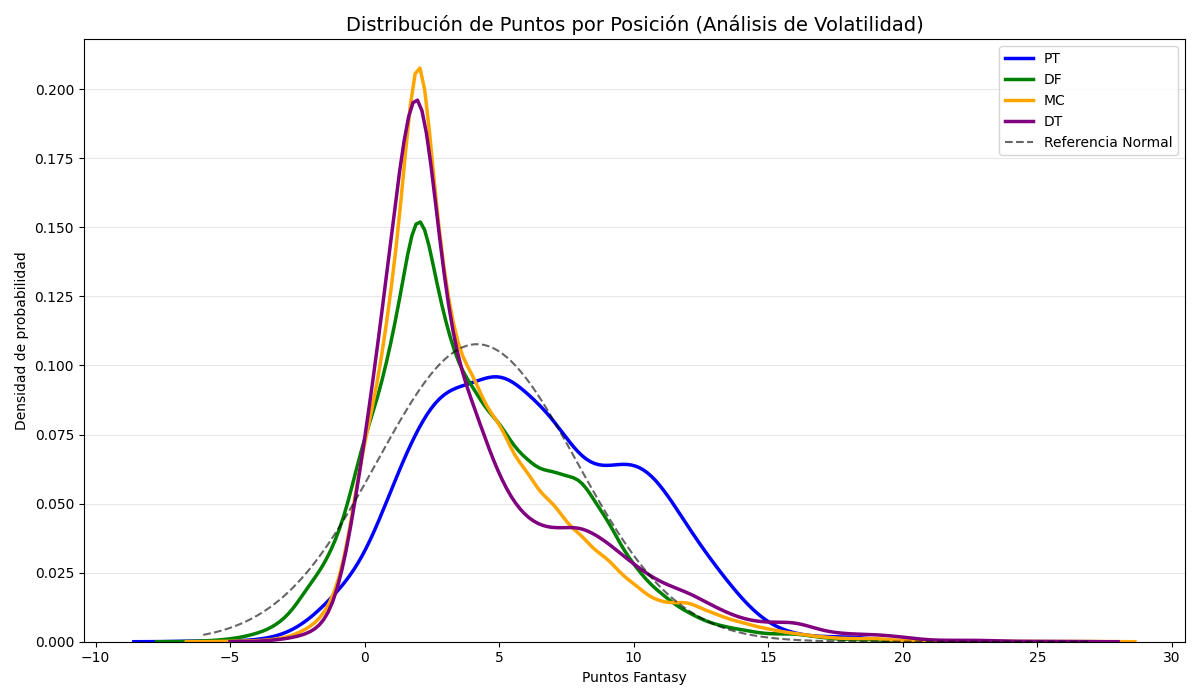
\includegraphics[width=0.8\textwidth]{images/normal.png}
\caption{Distribución de puntos por posición comparada con distribución normal.}
\label{fig:distribucion-puntos}
\end{figure}
 
\begin{itemize}
\item \textbf{Porteros (PT)}: Tienen una media de puntos más alta ($\approx 6.1$),
lo que permite un MAE absoluto mayor ($\approx 3.25$) manteniendo una fiabilidad
relativa alta (53.3\% de error).
\item \textbf{Centrocampistas y Defensas (MC/DF)}: Tienen medias más bajas
($\approx 3.9$), lo que implica que un error de 3 puntos supone casi un 71\% de
desviación sobre su media, siendo mucho más crítico reducir el error en estas
posiciones.
\end{itemize}
 
Para evitar los sesgos de los valores atípicos (jugadores con puntuaciones
extremas de 35 o 40 puntos), se ha descartado el uso de la desviación estándar
en favor de los percentiles de error.
 
Este enfoque garantiza que los umbrales de
validez se ajusten a la forma real de la distribución de cada posición.
A continuación, se presentan los objetivos de rendimiento que los modelos de
Machine Learning deben alcanzar para ser considerados válidos:
 
\begin{table}[H]
\centering
\renewcommand{\arraystretch}{1.3}
\begin{tabular}{|c|c|c|c|c|c|}
\hline
\textbf{Posición} & \textbf{Media} & \textbf{MAE} & \textbf{Error} &
\textbf{Excelente} & \textbf{Pobre} \\
& \textbf{Puntos} & \textbf{Medio} & \textbf{\%} & \textbf{(P25)} &
\textbf{(P75)} \\
\hline
PT & 6.09 & 3.25 & 53.3 & 2.93 & 3.63 \\
\hline
DF & 3.98 & 2.80 & 70.3 & 2.15 & 3.18 \\
\hline
MC & 3.94 & 2.81 & 71.2 & 2.10 & 3.25 \\
\hline
DT & 4.25 & 2.94 & 69.2 & 2.25 & 3.25 \\
\hline
\end{tabular}
\caption{Distribución de desempeño esperado por posición.}
\label{tab:benchmarking}
\end{table}
 
Por lo que los objetivos marcados para la fase de entrenamiento son:
 
\begin{table}[H]
\centering
\renewcommand{\arraystretch}{1.4}
\begin{tabular}{|c|c|c|c|}
\hline
\textbf{Posición} & \textbf{Élite (P25)} & \textbf{Aceptable} &
\textbf{Alerta (P75)} \\
& & \textbf{(Mediana)} & \\
\hline
Porteros (PT) & $MAE \le 2.93$ & $MAE \le 3.18$ & $MAE > 3.63$ \\
\hline
Defensas (DF) & $MAE \le 2.15$ & $MAE \le 2.79$ & $MAE > 3.18$ \\
\hline
Mediocentros (MC) & $MAE \le 2.10$ & $MAE \le 2.60$ & $MAE > 3.25$ \\
\hline
Delanteros (DT) & $MAE \le 2.25$ & $MAE \le 2.75$ & $MAE > 3.25$ \\
\hline
\end{tabular}
\caption{Objetivos de rendimiento para modelos de ML por posición.}
\label{tab:objetivos-ml}
\end{table}
 
\subsection{7.3 Decisiones de diseño estratégicas}
Más allá de la implementación técnica, el sistema incorpora una serie de
decisiones de diseño clave que afectan directamente a la validez, fiabilidad y
utilidad del modelo predictivo. Estas decisiones han sido tomadas considerando
tanto aspectos teóricos como prácticos del dominio.
En esta sección se exponen las principales elecciones estratégicas realizadas,
junto con su justificación y su impacto en el comportamiento del sistema.
 
\subsubsection{7.3.1 Estrategia de extracción y congelación de datos}
 
Se ha optado por congelar la extracción de datos en la jornada 17 de la
temporada 2025/26. Esta decisión se fundamenta en los siguientes pilares:
 
\begin{itemize}
\item \textbf{Volumen de datos significativo}: el histórico abarca 2 temporadas
y media de competición. Considerando una media de 25 jugadores con minutos por
cada uno de los 10 partidos de cada jornada, el volumen de registros gestionado
es superior a las 23.000 entradas. Este volumen garantiza una base estadística
sólida para el entrenamiento de los modelos.
 
\item \textbf{Factor de predicción real}: al limitar el entrenamiento hasta la
jornada 17, el sistema se enfrenta a datos que ``desconoce'' (las jornadas
posteriores). Esto permite realizar un backtesting funcional genuino, donde el
modelo debe predecir resultados que, aunque ya han ocurrido en la realidad, no
han sido utilizados para su ajuste.
 
\item \textbf{Integridad del modelo}: aunque se han
implementado técnicas de ingeniería de variables para evitar que información del
futuro se filtre en el pasado, la decisión de realizar un corte temporal
estricto actúa como una salvaguarda física. De este modo, se asegura que el
modelo solo toma decisiones basadas en la información que un mánager real
tendría disponible en el momento de realizar su alineación.
\end{itemize}
 
\subsubsection{7.3.2 Especialización de modelos por posición}
 
Una de las innovaciones clave en la arquitectura es la segmentación del
aprendizaje según el rol del jugador. Se ha descartado el uso de un modelo único
global en favor de modelos específicos para cada demarcación (Porteros,
Defensas, Centrocampistas y Delanteros).
 
Esta decisión se fundamenta en la heterogeneidad de las métricas de rendimiento:
 
\begin{itemize}
\item \textbf{Divergencia de variables}: las variables que determinan el éxito de
un Portero (PT), como paradas, despejes o goles encajados, son irrelevantes o
inexistentes para un Mediocentro (MC), quien se evalúa por pases clave,
recuperaciones o asistencias.
 
\item \textbf{Distribución de puntuaciones}: los sistemas de puntuación ponderan
de forma distinta las mismas acciones según la posición. Un gol de un defensa
suele tener un impacto estadístico y de puntuación mayor que el de un delantero.
 
\item \textbf{Optimización del aprendizaje}: al entrenar modelos independientes,
el algoritmo de boosting puede identificar patrones específicos de cada posición
sin el ``ruido'' que generarían los perfiles estadísticos de otros roles. Esto
reduce el error absoluto medio (MAE) y mejora la precisión en jugadores con
roles muy específicos.
\end{itemize}
 
Se observan diferencias significativas en la distribución de puntos según la
posición, por lo que se considera esta opción más adecuada para aportar valor
y abordar el problema de la forma más realista posible.
 
\subsection{7.4 Modelado de datos}
El diseño de los datos constituye uno de los pilares fundamentales del sistema,
ya que determina tanto la integridad de la información como la eficiencia en su
acceso y procesamiento. Para ello, se ha seguido un enfoque progresivo que
abarca desde el modelo conceptual hasta su implementación en base de datos.
 
En este apartado se describe la evolución del modelo de datos a través de sus
distintos niveles de abstracción, garantizando la coherencia entre el diseño
teórico y la implementación final.
 
El diseño de la base de datos se ha desarrollado de forma progresiva a través de
tres niveles de abstracción: modelo conceptual, modelo entidad-relación (ER) y
modelo lógico. Esta evolución permite partir de una visión general del dominio
hasta llegar a una implementación concreta en base de datos, alineada finalmente
con los modelos definidos en Django (models.py).
 
\subsubsection{7.4.1 Modelado conceptual}
El modelo conceptual define las entidades principales del dominio y las
relaciones entre ellas a alto nivel, sin entrar aún en detalles de
implementación. En este caso, el dominio modelado corresponde a una competición
de fútbol con información tanto estructural (equipos, jornadas, partidos) como
analítica (estadísticas y rendimiento de jugadores).
 
Las entidades principales identificadas son:
 
\begin{itemize}
\item \textbf{Temporada}: representa una competición concreta (por ejemplo,
2023/2024). Es el eje central del modelo.
\item \textbf{Equipo}: entidad independiente que participa en distintas
temporadas.
\item \textbf{Jugador}: entidad que representa a cada futbolista.
\item \textbf{Jornada}: subdivisión temporal de una temporada.
\item \textbf{Partido}: evento en el que participan dos equipos dentro de una
jornada.
\end{itemize}
 
A partir de estas entidades principales, se introducen entidades intermedias y
de análisis:
 
\begin{itemize}
\item \textbf{EquipoTemporada}: resuelve la relación muchos-a-muchos entre
equipo y temporada.
\item \textbf{EquipoJugadorTemporada}: representa la plantilla de un equipo en
una temporada concreta, incluyendo atributos como dorsal, edad o percentiles.
\item \textbf{ClasificacionJornada}: almacena la clasificación de los equipos
en cada jornada.
\item \textbf{EstadisticasPartidoJugador}: recoge el rendimiento individual de
cada jugador en un partido.
\item \textbf{Calendario}: estructura auxiliar para consultas rápidas de
partidos programados.
\item \textbf{RendimientoHistoricoJugador}: agrega estadísticas acumuladas por
jugador, equipo y temporada.
\end{itemize}
 
\textbf{Relaciones clave del modelo conceptual:}
 
\begin{itemize}
\item Una Temporada contiene múltiples Jornadas.
\item Una Temporada tiene múltiples Equipos (a través de EquipoTemporada).
\item Un Equipo participa en múltiples Partidos.
\item Un Jugador juega en múltiples equipos y temporadas (a través de
EquipoJugadorTemporada).
\item Un Partido genera estadísticas de múltiples jugadores.
\item Un Jugador tiene historial y estadísticas acumuladas.
\end{itemize}
 
\begin{figure}[H]
\centering
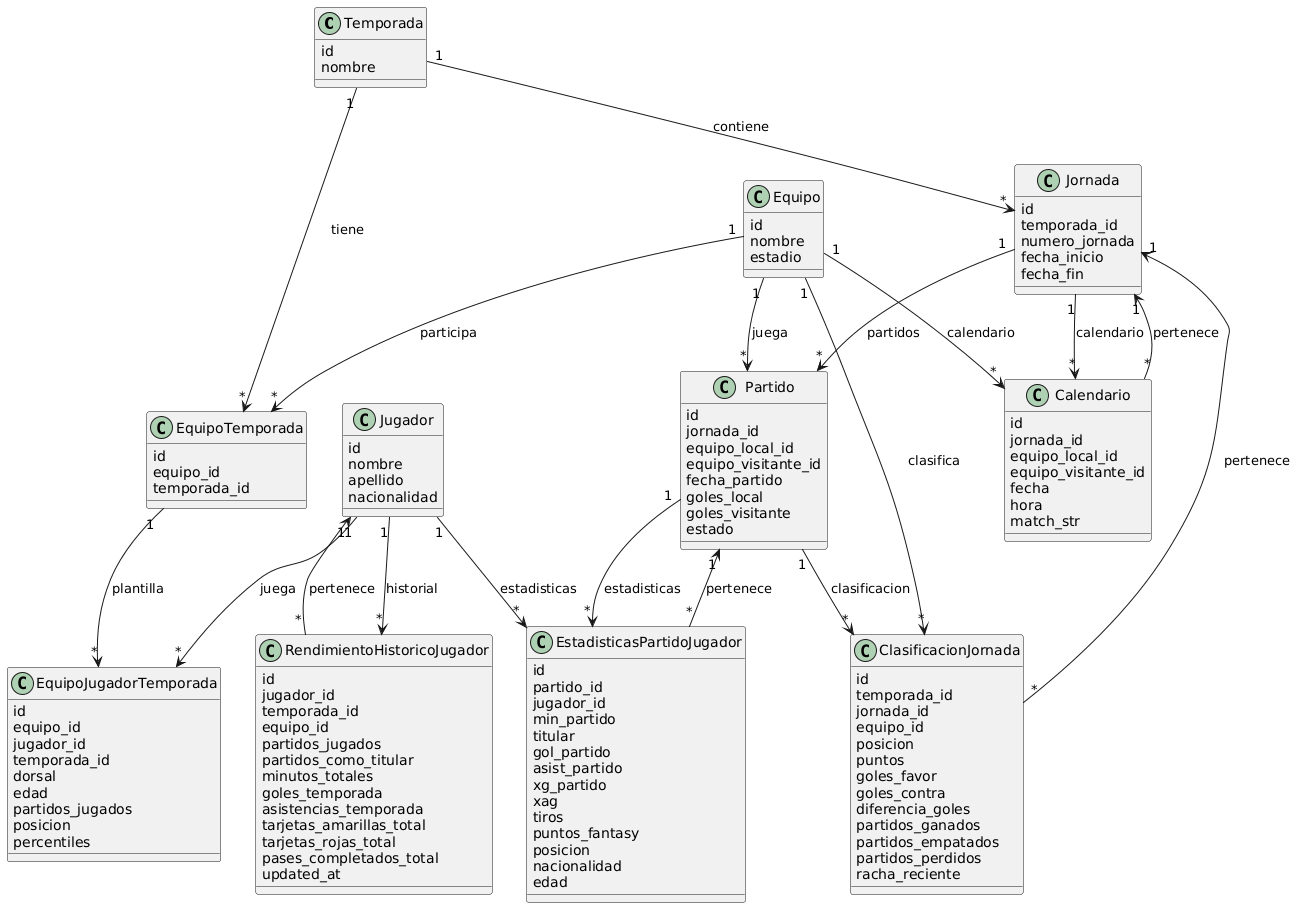
\includegraphics[width=0.8\textwidth]{images/modeloconceptual.png}
\caption{Modelo conceptual del sistema.}
\label{fig:modelo-conceptual}
\end{figure}
 
\subsubsection{7.4.2 Diagrama entidad-relación}
Dando el salto natural a la arquitectura relacional, el segundo diagrama elimina
el ruido visual de los atributos para centrarse exclusivamente en cómo las
entidades interactúan entre sí, observándose claramente las cardinalidades.
 
\textbf{Relaciones principales:}
 
\begin{itemize}
\item Una temporada contiene múltiples jornadas, mientras que cada jornada
pertenece a una única temporada.
\item Una temporada se asocia con múltiples registros de equipo-temporada, lo que
permite modelar la participación de distintos equipos en cada edición de la
competición. Esta relación resuelve el caso muchos-a-muchos entre equipos y
temporadas.
\item Un equipo participa en múltiples partidos, ya sea como equipo local o
visitante.
\item Una jornada agrupa múltiples partidos.
\item Un partido genera múltiples registros en estadísticas de partido por jugador.
\item Un jugador puede tener múltiples registros de estadísticas de partido,
correspondientes a los distintos eventos.
\item La entidad equipo-temporada se relaciona con equipo-jugador-temporada, lo que
permite definir la plantilla de cada equipo en una temporada concreta, incluyendo
información adicional como dorsal, edad o métricas avanzadas.
\item Un jugador se relaciona con rendimiento histórico, lo que permite almacenar
estadísticas agregadas por temporada y equipo, facilitando el análisis
longitudinal de su rendimiento.
\end{itemize}
 
\begin{figure}[H]
\centering
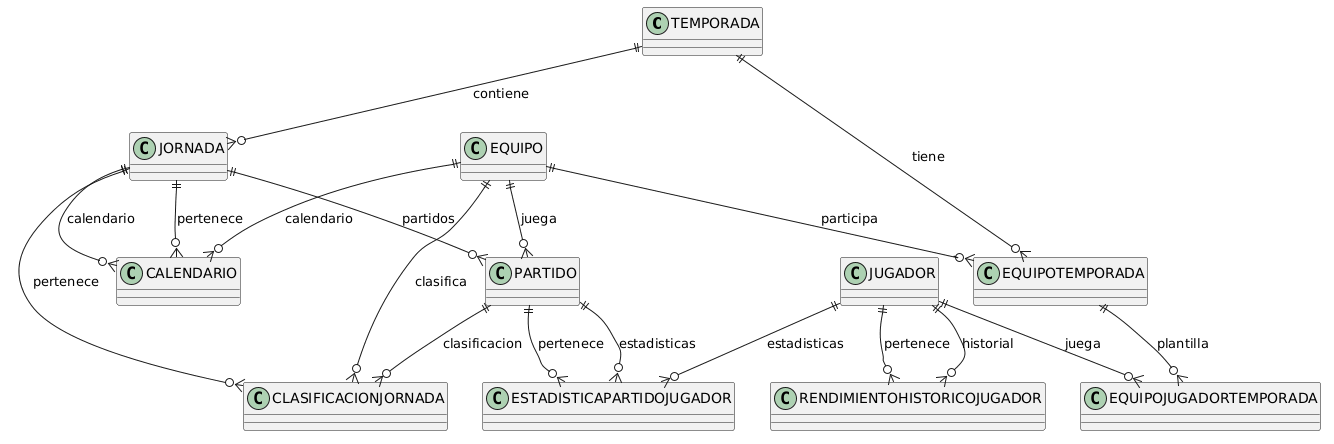
\includegraphics[width=0.8\textwidth]{images/diagramaer.png}
\caption{Diagrama Entidad-Relación.}
\label{fig:diagrama-er}
\end{figure}
 
\subsubsection{7.4.3 Modelo lógico}
El modelo lógico representa la implementación concreta en base de datos
relacional, y en este caso se ha desarrollado directamente a partir de Django
(models.py), lo cual garantiza coherencia entre diseño e implementación.
 
Cada entidad del modelo ER se transforma en una tabla (entity) con:
 
\begin{itemize}
\item Clave primaria (id)
\item Claves foráneas (FK)
\item Restricciones (UNIQUE, validators)
\end{itemize}
 
El modelo lógico no es solo teórico, sino que está implementado directamente en
Django:
 
\begin{itemize}
\item Cada entidad $\rightarrow$ models.Model
\item Relaciones $\rightarrow$ ForeignKey
\item Restricciones $\rightarrow$ unique\_together, validators
\item Enumeraciones $\rightarrow$ TextChoices (ej: EstadoPartido, Posicion)
\end{itemize}
 
\begin{figure}[H]
\centering
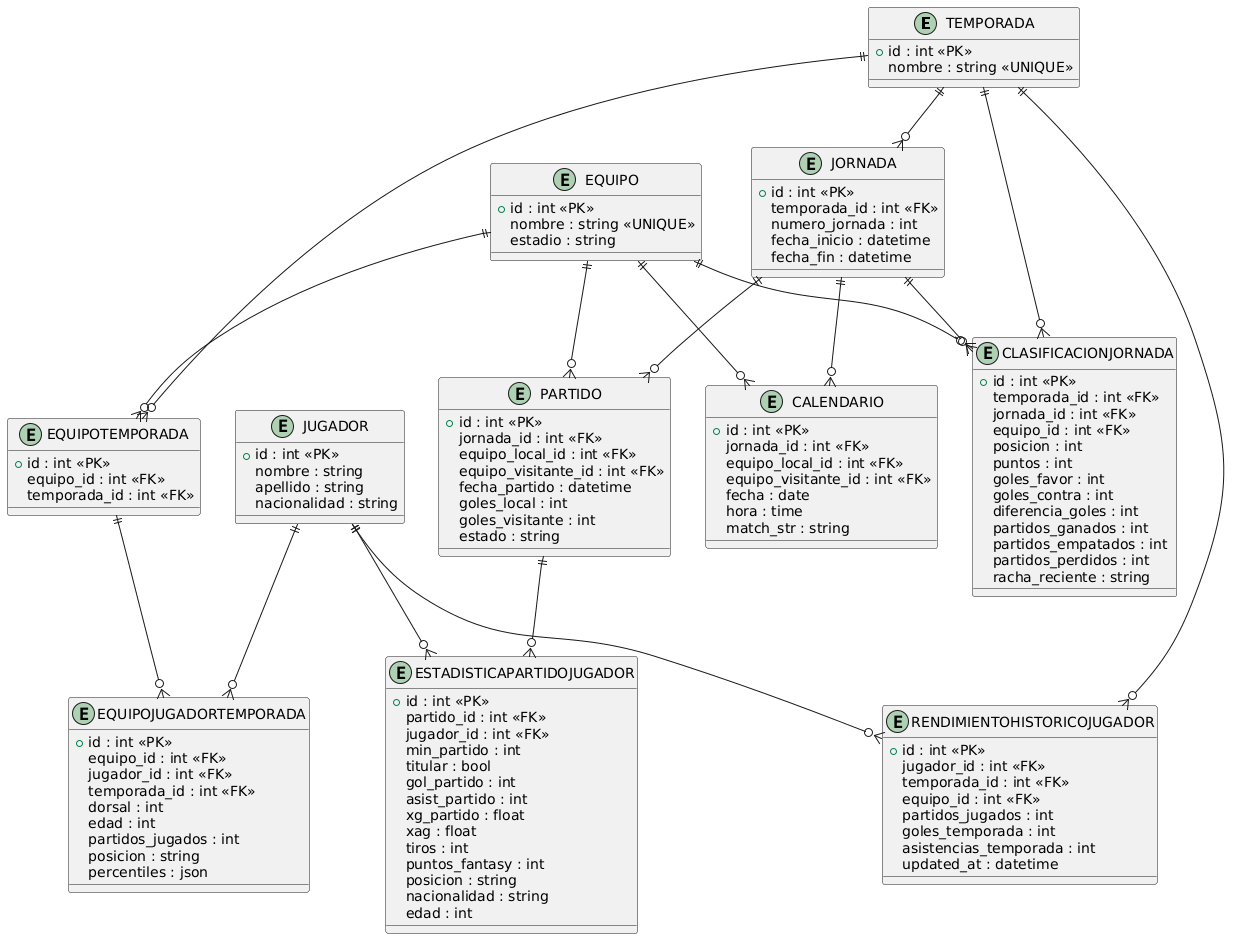
\includegraphics[width=0.8\textwidth]{images/esquemalogico.png}
\caption{Esquema lógico del sistema.}
\label{fig:esquema-logico}
\end{figure}
 
\subsection{7.5 Infraestructura de datos y búsqueda}
Con el fin de cumplir los requisitos de rendimiento y escalabilidad, el sistema
se apoya en una infraestructura de datos compuesta por múltiples tecnologías
especializadas, ya explicada en el punto de Stack Tecnológico. Cada una de ellas
 desempeña un papel fundamental en la gestión,
consulta y optimización de la información.
 
En esta sección se describen los distintos sistemas utilizados, así como su
integración dentro de la arquitectura global y la justificación de su elección.
 
\begin{itemize}
\item \textbf{Base de datos (PostgreSQL)}: Es el sistema de persistencia
relacional primario. Almacena la información estructural y crítica: datos de
jugadores, histórico de plantillas, usuarios y configuraciones de seguridad.
Garantiza la integridad referencial y el cumplimiento de las propiedades ACID.
 
\item \textbf{MeiliSearch}: Se utiliza como motor de indexación y búsqueda
avanzada. Su función es permitir que el Buscador (RF4) y el Matching de
entidades funcionen con latencias mínimas, incluso sobre grandes volúmenes de
texto, mediante el uso de índices invertidos.
 
\item \textbf{Redis}: Actúa como capa de memoria distribuida de alta velocidad y
como infraestructura de mensajería interna. En el sistema se utiliza para
cachear respuestas frecuentes de la API y para soportar el canal de comunicación
de Django Channels en funcionalidades en tiempo real. Esta doble función reduce
la carga de PostgreSQL y estabiliza la latencia en operaciones repetitivas, a la
vez que garantiza coordinación entre instancias backend.
\end{itemize}
 
Inicialmente, se consideró el uso de Elasticsearch como motor de búsqueda. Sin
embargo, debido a las limitaciones de licencia y a la necesidad de utilizar una
solución completamente abierta y sin costes asociados, se decidió sustituirlo
por OpenSearch. Esta alternativa, desarrollada como un fork open source de
Elasticsearch, mantiene una alta compatibilidad a nivel conceptual y funcional,
permitiendo implementar las mismas estrategias de indexación y consulta sin
dependencia de licencias propietarias. Finalmente, esta opción se descartó debido
a motivos de rendimiento y se sustituyó por MeiliSearch.
 
\subsection{7.7 Diseño de la interfaz}
La interfaz de usuario constituye el punto de interacción entre el sistema y el
usuario final, por lo que su diseño debe garantizar tanto la usabilidad como la
claridad en la presentación de la información.
En esta sección se describe la estructura de navegación, los componentes
principales y las decisiones de diseño visual adoptadas, con el objetivo de
ofrecer una experiencia de usuario coherente e intuitiva.
 
\subsubsection{7.7.1 Nivel de navegación}
 
El nodo raíz o vista de aterrizaje es el Menú (Home). Desde este punto, o a
través del Sidebar, el sistema bifurca la navegación hacia los diferentes
dominios de la aplicación:
 
\begin{itemize}
\item \textbf{Clasificación}: vista general del estado de la liga y resultados de
la jornada seleccionada.
\item \textbf{Vista Jugador}: acceso directo a perfiles individuales.
\item \textbf{Mi Plantilla}: módulo de gestión del equipo del usuario.
\item \textbf{Amigos}: módulo social para interactuar con otros usuarios.
\item \textbf{Equipos}: directorio o listado global de las entidades deportivas.
\end{itemize}
 
\subsubsection{7.7.2 Estructura base y componentes persistentes}
 
La interfaz se construye sobre un layout principal que encapsula dos componentes
de renderizado persistente, garantizando que el usuario nunca pierda el contexto
de navegación:
 
\begin{itemize}
\item \textbf{Navbar (barra de navegación superior)}: Actúa como el controlador
del estado de autenticación de la sesión. Es visible en todas las rutas de la
aplicación y renderiza condicionalmente el acceso al inicio de sesión (Login) o
la gestión de la cuenta (Perfil), dependiendo de la sesión activa del usuario.
\item \textbf{Sidebar (menú lateral)}: Funciona como el enrutador principal
(NavHost). Está permanentemente accesible y proporciona saltos directos a los
módulos core del sistema: Menú, Mi Plantilla, Liga, Amigos, Equipos y Estadísticas.
\end{itemize}
 
\subsubsection{7.7.3 Flujos de profundización}
 
La aplicación implementa un sistema de navegación jerárquica donde las vistas
generales actúan como pasarelas hacia vistas de detalle, pasando los
identificadores correspondientes (por ejemplo, vía parámetros en la URL o props
en el enrutador):
 
\begin{itemize}
\item \textbf{Flujo de entidades deportivas}: tanto la vista de Clasificación
como el directorio general de Equipos convergen en un nodo común: el Detalle de
Equipo. A su vez, el Detalle de Equipo actúa como contenedor de una plantilla,
permitiendo navegar hacia la Vista Jugador específica al seleccionar un
integrante del club.
\item \textbf{Flujo analítico}: la vista de Estadísticas permite el salto directo
hacia la Vista Jugador para consultar métricas detalladas de un perfil concreto.
\item \textbf{Flujo social}: la vista de Amigos permite ramificar la navegación
hacia el Detalle de Amigo. Por otro lado, la vista de Mi Plantilla no contiene
navegación específica más allá del navbar y el menú lateral.
\end{itemize}
 
\begin{figure}[H]
\centering
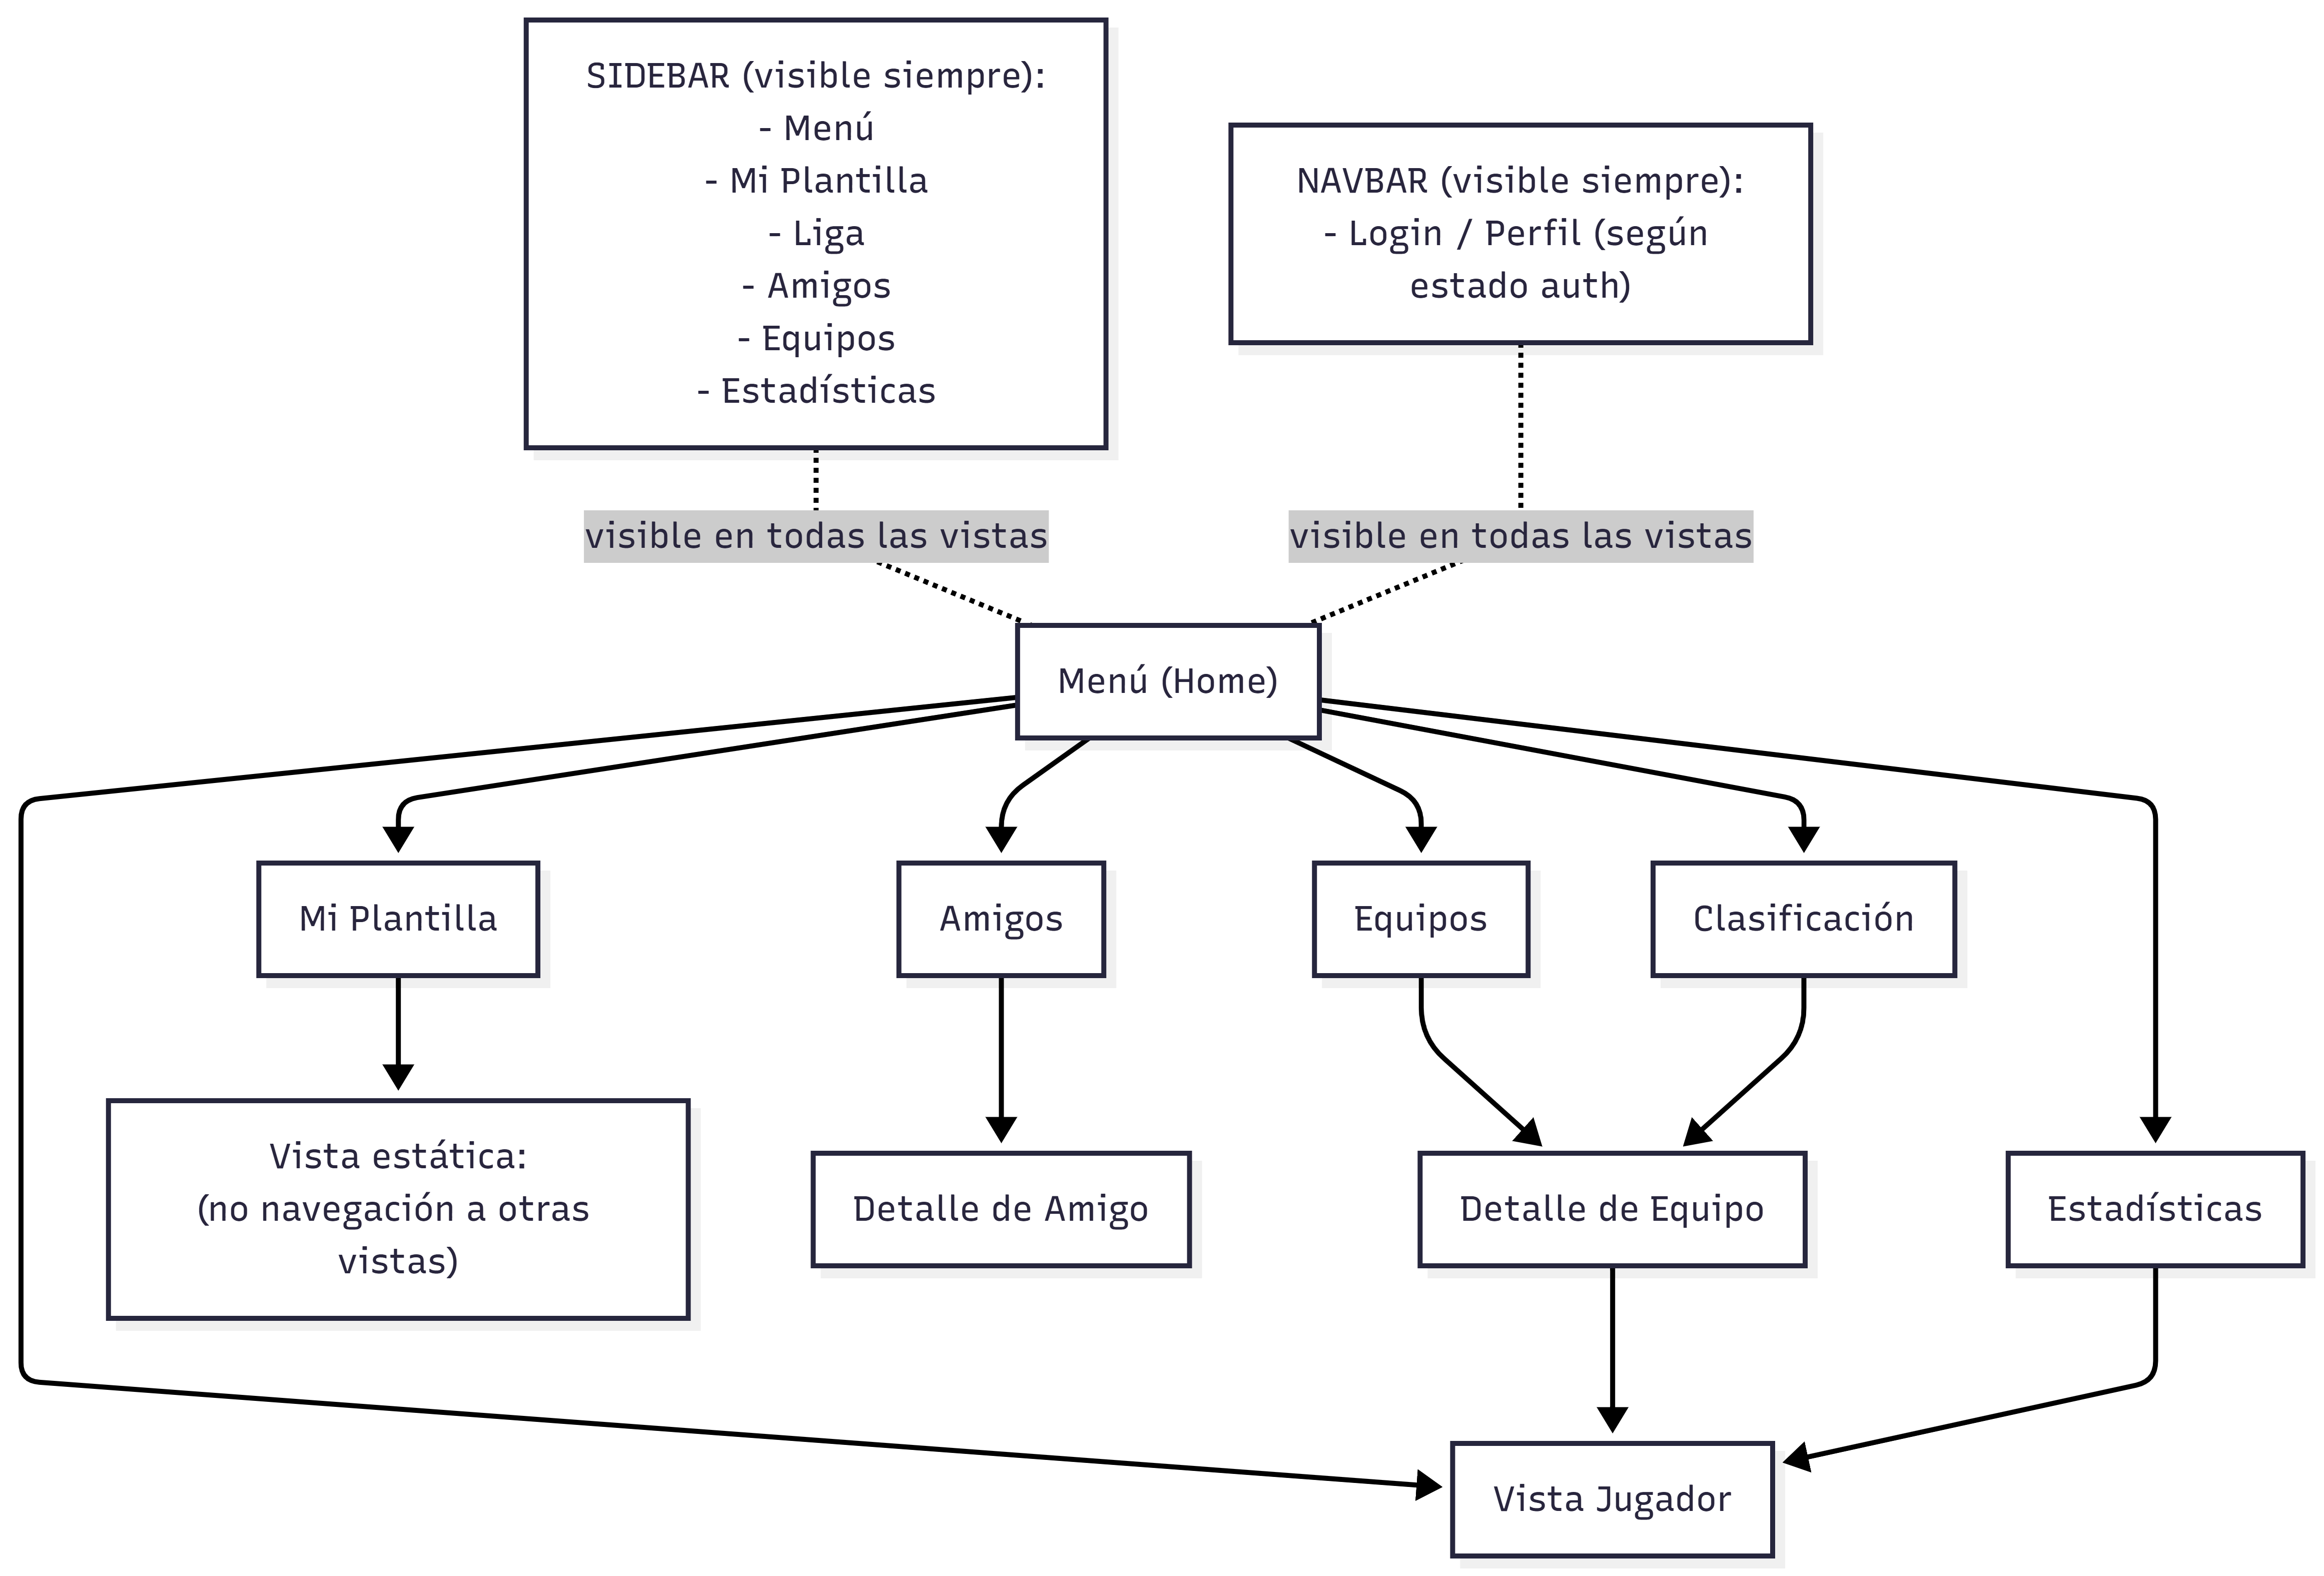
\includegraphics[width=0.8\textwidth]{images/navegacion.png}
\caption{Diagrama de navegación de UI.}
\label{fig:nav-ui}
\end{figure}
 
\subsubsection{7.7.4 Diseño de la interfaz}
El diseño de la paleta de colores responde a criterios de simplicidad, contraste y coherencia visual.
La combinación de verde vibrante (\textit{Primary}) con tonalidades más oscuras busca transmitir una sensación
de tecnología, modernidad e innovación, valores que se alinean
con la naturaleza inteligente del sistema y su integración con modelos de Machine Learning e IA.
 
\begin{table}[H]
\centering
\renewcommand{\arraystretch}{2.5}
\begin{tabular}{|c|c|c|c|c|}
\hline
\textbf{Primary} & \textbf{Primary dark} & \textbf{Negro puro} & \textbf{Gris oscuro} & \textbf{Gris dark} \\
\hline

\includegraphics[width=0.15\textwidth,height=1cm]{images/colores/primary.png} &

\includegraphics[width=0.15\textwidth,height=1cm]{images/colores/darkprimary.png} &

\includegraphics[width=0.15\textwidth,height=1cm]{images/colores/negropuro.png} &

\includegraphics[width=0.15\textwidth,height=1cm]{images/colores/grisoscuro.png} &

\includegraphics[width=0.15\textwidth,height=1cm]{images/colores/grisdark.png} \\
\hline
\small \#50c878 & \small \#2d8659 & \small \#050505 & \small \#1e1e1e & \small \#262626 \\
\hline
\end{tabular}
\caption{Paleta de colores empleada en la interfaz.}
\label{fig:colores-marca}
\end{table}
 
\paragraph*{Familia tipográfica}
 
\begin{itemize}
\item \textbf{Display}: Lexend, sans-serif (títulos y elementos destacados)
\item \textbf{Body}: Noto Sans, sans-serif (textos corridos y descripciones)
\end{itemize}
 
\subsection{7.8 Diseño de seguridad y autenticación}
El sistema implementa la seguridad utilizando las capacidades nativas de Django,
lo que incluye autenticación basada en sesiones, protección frente a ataques
CSRF, gestión segura de cookies y almacenamiento de contraseñas mediante
algoritmos de hashing robustos. Esta aproximación permite delegar en el
framework gran parte de la gestión de la seguridad, reduciendo la complejidad
del desarrollo y minimizando errores comunes en la implementación manual de
estos mecanismos.
 
\subsection{7.9 Diseño del despliegue}
Para garantizar la portabilidad, escalabilidad y consistencia del sistema entre
los diferentes entornos de ejecución, se ha adoptado una estrategia de
containerización basada en Docker y Docker Compose. Esta decisión permite aislar
las dependencias de cada componente, asegurando que el software se comporte de
manera idéntica en desarrollo, preproducción y producción.
 
\subsubsection{7.9.1 Ecosistema de contenedores y responsabilidades}
 
Durante el desarrollo, el sistema se descompone en cinco servicios principales orquestados mediante una
red virtual privada:
 
\begin{itemize}
\item \textbf{Capa de persistencia (db)}: basada en PostgreSQL 16-alpine. Se ha
seleccionado la variante alpine para minimizar el peso de la imagen. La
persistencia se garantiza mediante volúmenes de Docker (postgres\_data).
\item \textbf{Capa de caché y mensajería (redis)}: basada en Redis 7 alpine.
Proporciona caché distribuida para respuestas de API y backend de channel layer
para Django Channels. Su incorporación reduce latencia en lecturas repetidas y
permite comunicación en tiempo real entre múltiples instancias del backend.
\item \textbf{Motor de búsqueda (meilisearch)}: nodo de MeiliSearch
encargado de la indexación y consultas de alto rendimiento.
\item \textbf{Núcleo de aplicación (backend)}: ejecuta la lógica de Django
sobre un servidor Daphne (ASGI), permitiendo la gestión híbrida de peticiones
REST y comunicaciones bidireccionales mediante WebSockets.
\item \textbf{Servidor web y frontend (frontend)}: contenedor dual que contiene
los assets de React y un servidor Nginx configurado como punto de entrada único
al sistema.
\end{itemize}
 
\begin{figure}[H]
\centering
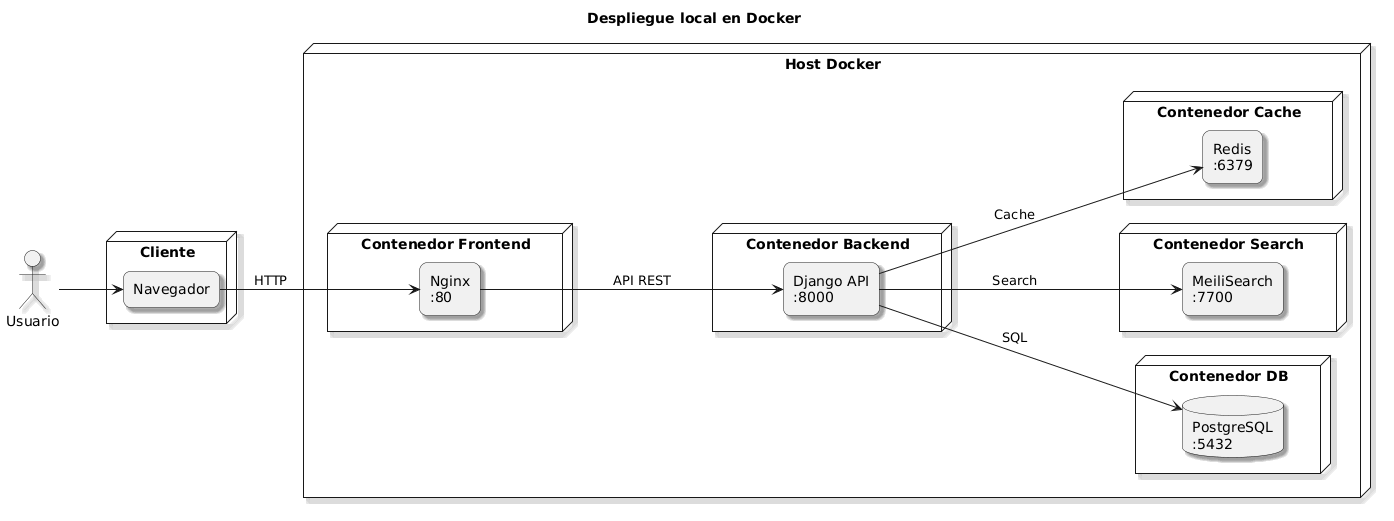
\includegraphics[width=0.8\textwidth]{images/despliegue-local.png}
\caption{Diagrama de despliegue del sistema en local.}
\label{fig:despliegue-local}
\end{figure}
 
Para la fase de producción, se ha optado por una estrategia diferente: utilizar servicios gestionados en la nube para
alojar la base de datos, la capa de caché y el frontend. Esta decisión ha sido motivada por el uso del crédito de Azure
proporcionado por la Universidad de Sevilla; si se desplegaba todo en conjunto, el rendimiento era deficiente y se consumiría todo
el crédito disponible en poco tiempo.
 
\begin{figure}[H]
\centering
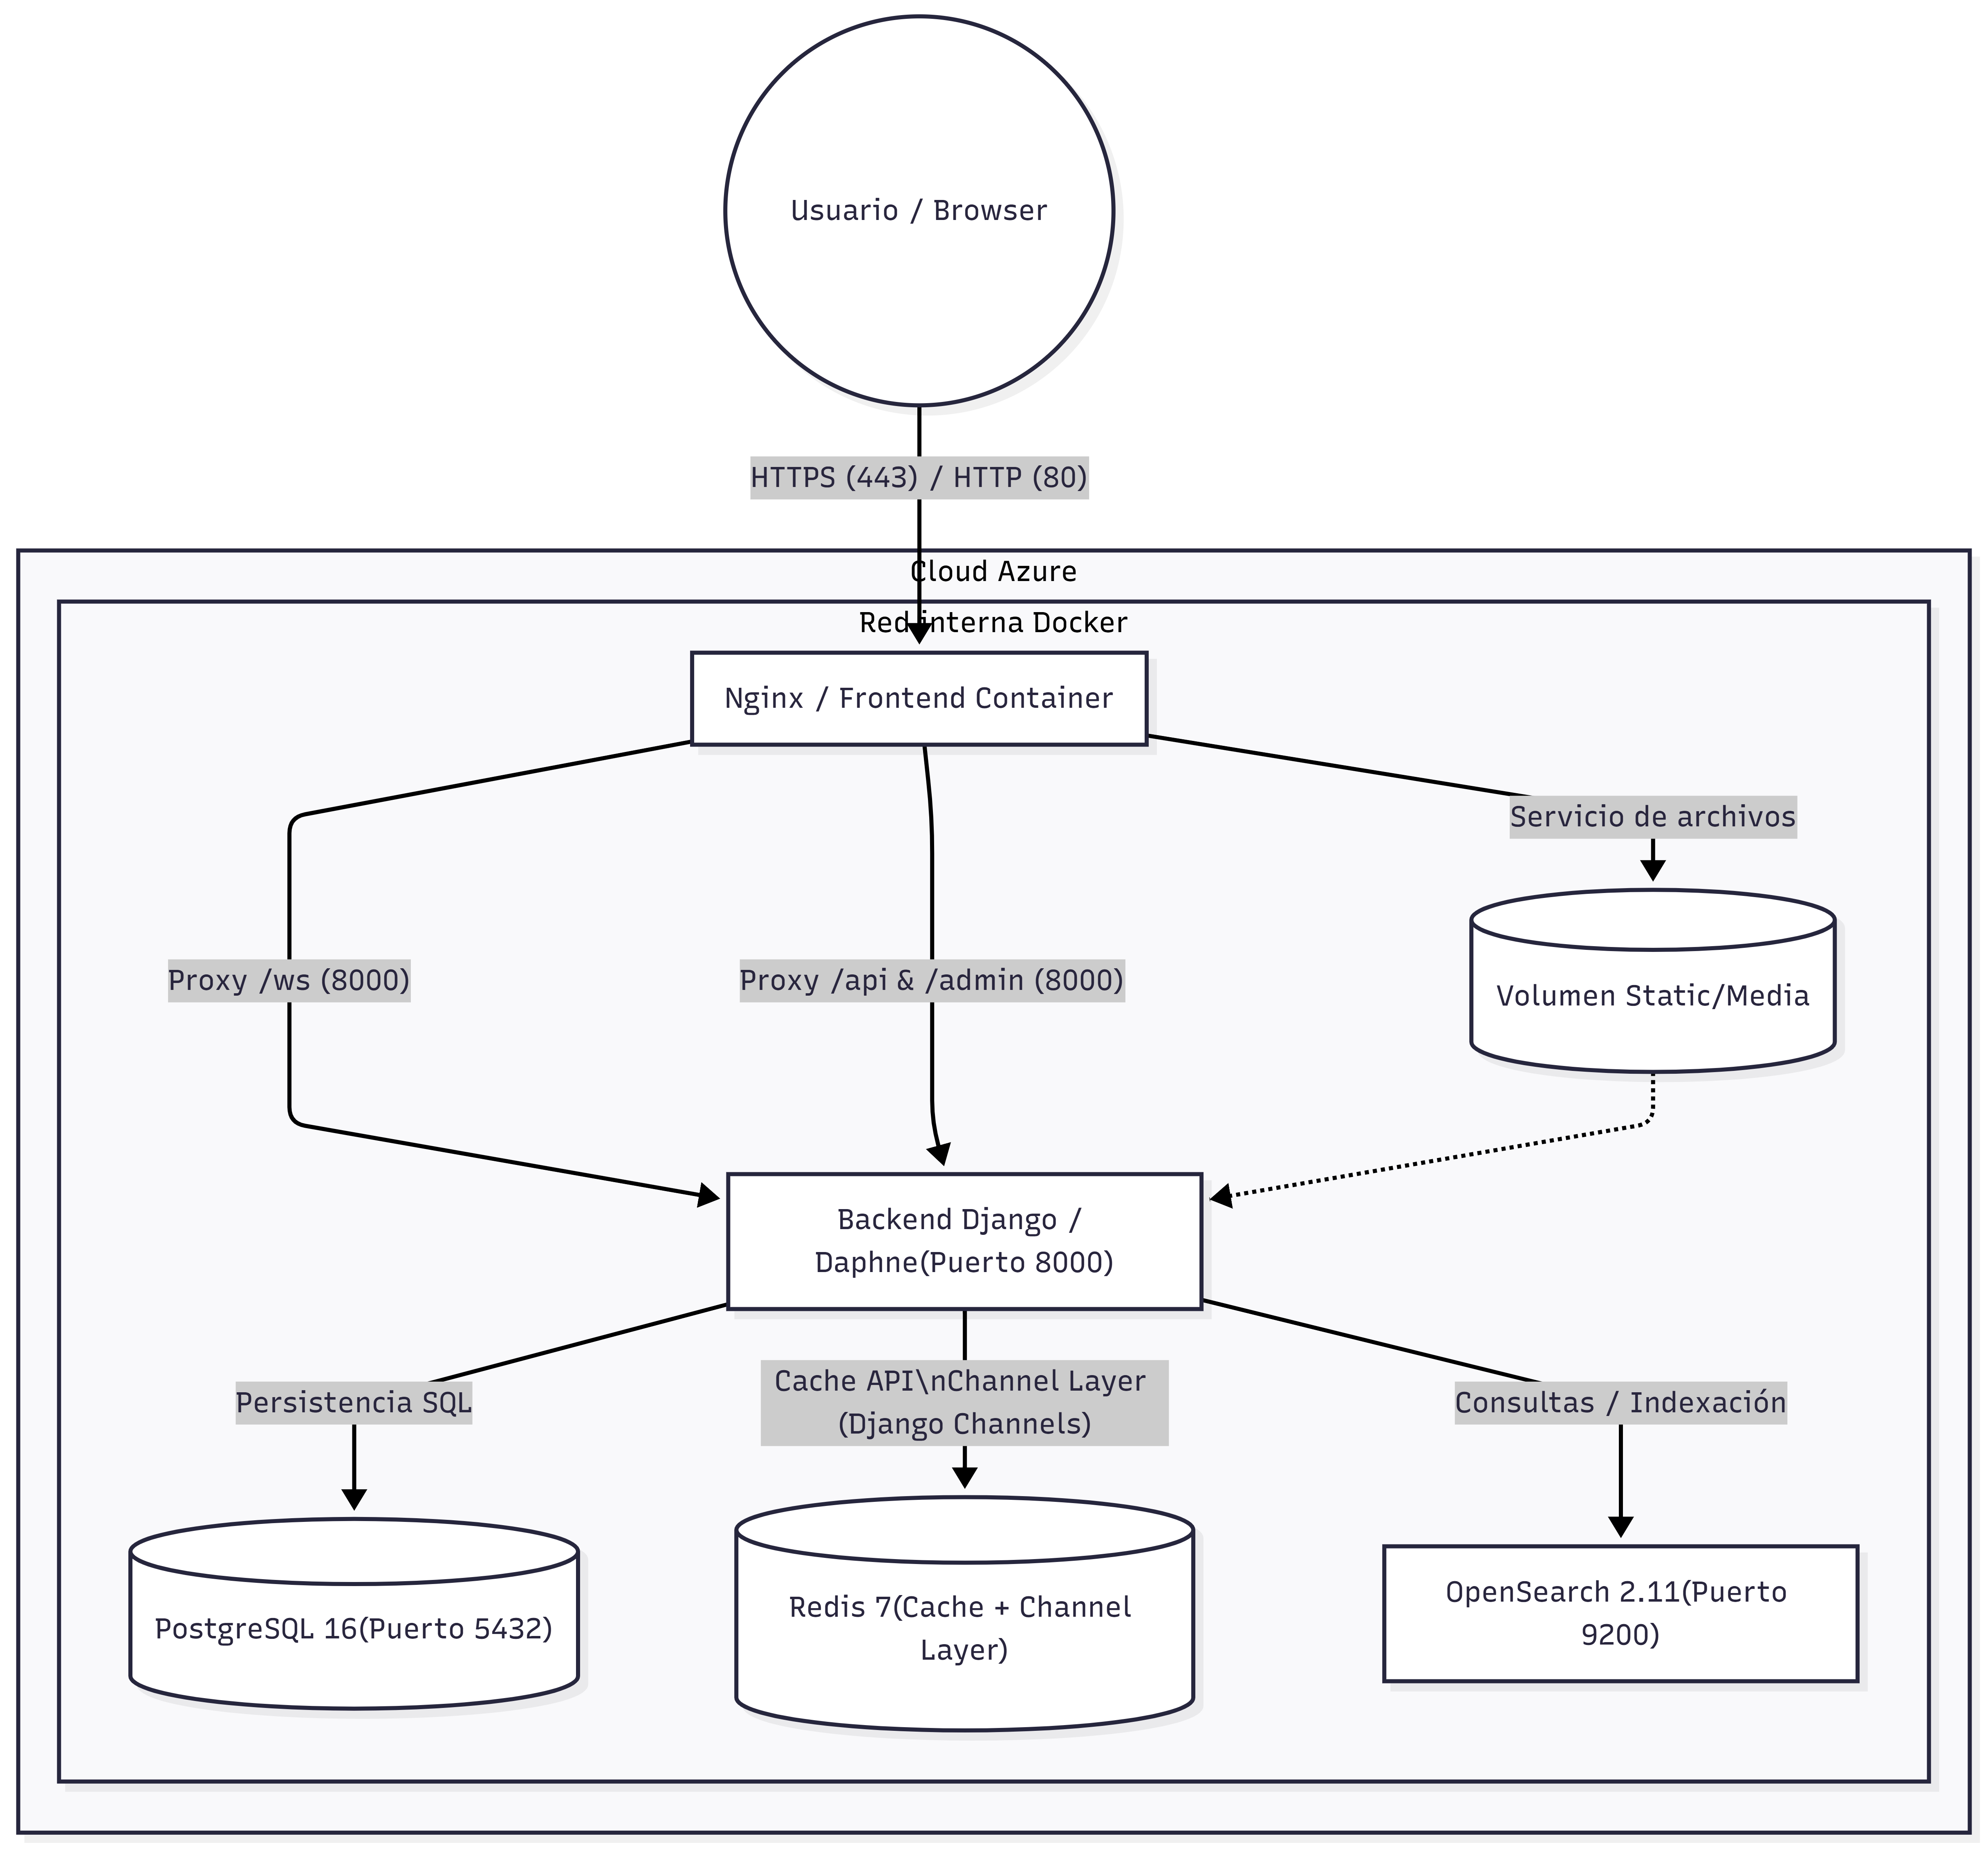
\includegraphics[width=0.8\textwidth]{images/diagramadespliegue.png}
\caption{Diagrama de despliegue del sistema en fase de producción.}
\label{fig:despliegue}
\end{figure}
 
\subsubsection{7.9.2 Estrategia de construcción}
 
Para optimizar el rendimiento y la seguridad, se han diseñado Dockerfiles
multi-etapa:
 
\begin{itemize}
\item \textbf{Backend}: se utiliza una primera etapa (builder) con las
herramientas de compilación necesarias para instalar las dependencias de
Python y las librerías de Machine Learning. En la etapa de runtime, solo se
copian los binarios instalados a una imagen limpia de Python 3.11-slim,
reduciendo drásticamente el tamaño final y eliminando herramientas de
compilación que podrían ser explotadas.
\item \textbf{Frontend}: se emplea un entorno Node.js 20-slim para la
construcción con React. Posteriormente, el resultado se transfiere a una imagen
de Nginx Alpine, que actúa como servidor de alto rendimiento para archivos
estáticos.
\end{itemize}
 
Se han definido dos entornos diferenciados para cubrir el ciclo de
desarrollo:
 
\begin{itemize}
\item \textbf{Entorno de desarrollo (Local)}: ejecución mediante docker-compose
up en la máquina local del desarrollador. Permite una depuración rápida
manteniendo la paridad con el entorno final.
\item \textbf{Entorno de producción (Azure)}: el despliegue final se realiza en
Azure Web App for Containers. Esta elección permite escalar vertical y
horizontalmente el sistema según la carga de usuarios. Se aprovecha el crédito
ofrecido por la Universidad de Sevilla a través del programa Azure for Students,
garantizando un entorno profesional, seguro y monitorizado sin coste adicional
para el proyecto.
\end{itemize}
 
En definitiva, la estrategia de despliegue se ha regido por un principio de
optimización crítica de recursos sin sacrificio de funcionalidad.
La selección sistemática de versiones slim y alpine para las imágenes base, junto con una
configuración de contenedores de baja demanda, permite ofrecer la experiencia de
usuario completa y el rendimiento analítico requerido manteniendo una huella
computacional mínima. Este enfoque garantiza la viabilidad del sistema dentro de
los límites de computación del programa Azure for Students, evitando el
agotamiento prematuro de las cuotas de crédito de la Universidad de Sevilla.